\section{Evaluation}
\subsection{}

\begin{frame}
  \frametitle{Cloud Environment}
  Cloud with 6 identical computers running Hadoop 2.4, each with following specs:
  \begin{itemize}
    \item Intel Core2 Duo CPU E8200 @ \unit[2.66]{GHz} (2$\times$\unit[2.66]{GHz}, no hyperthreading)
    \item \unit[6]{MB} shared L2 cache, \unit[32]{KB} L1 data cache, \unit[32]{KB} L1 instruction cache
    \item \unit[4]{GB} (2$\times$\unit[2]{GB}) DDR2 RAM @ \unit[667]{MHz}
    \item \unit[64]{Bit} Ubuntu Linux 14.04.1 LTS with kernel 3.13.0-37
  \end{itemize}
  \vspace{1em}
  Computers connected to \unit[1]{Gb} Ethernet switch
\end{frame}

% \begin{frame}
%   \frametitle{Evaluation}
%   Methodology:
%   \begin{itemize}
%     \item Measure algorithm execution time for 1 worker $\rightarrow$ basis for evaluation
%     \item Increase parallel worker sizes from 1 to 15 to evaluate speedup
%     \item Compare parallel execution times to execution time of standalone algorithm implementation (no Hadoop, no other framework)
%   \end{itemize}
% \end{frame}

% \begin{frame}
%   \frametitle{Algorithms and benchmark problems}
%   \begin{itemize}
%     \item Implement bio - inspired optimization algorithms to solve benchmark problems
%     \item Execute benchmarks
%     \item Evaluate accuracy
%   \end{itemize}
% \end{frame}

\begin{frame}
  \frametitle{Implemented Algorithms and benchmark problems} 
  \begin{itemize}
    \item NSGA-II to solve Zitzler-Deb-Thiele's function nr. 3 (ZDT-3): solution evaluation not compute intense
    \item GA to solve tiled matrix multiplication (TMM): solution evaluation is computational intense
%     \item Evaluation of solutions is computed on workers
  \end{itemize}
  \scriptsize
  \begin{columns}
    \begin{column}{.5\textwidth}
      \begin{center}
	ZDT-3
	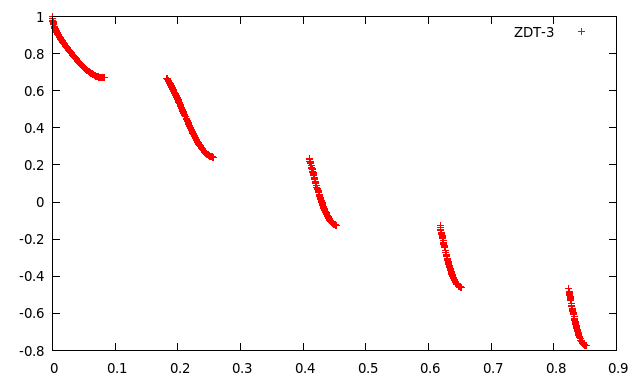
\includegraphics[width=50mm]{zdt3.png}
      \end{center}
    \end{column}
    \begin{column}{.5\textwidth}
      \begin{center}
	TMM\\
	\vspace{.5em}
	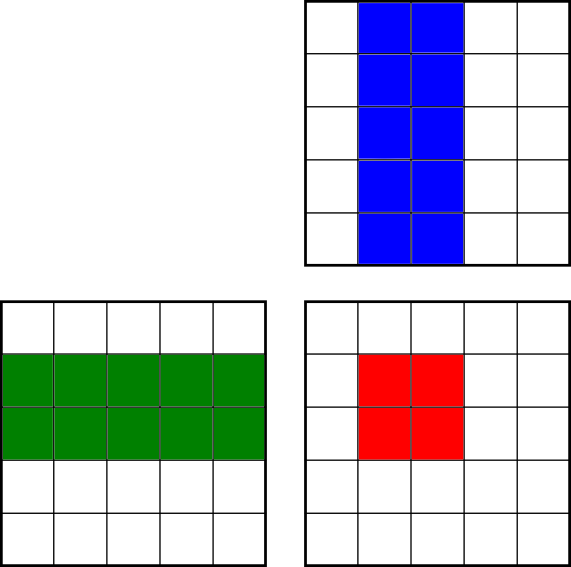
\includegraphics[width=30mm]{tmm.png}
      \end{center}
    \end{column}
  \end{columns}
\end{frame}

% \begin{frame}
%   \frametitle{Implemented Algorithms and benchmark problems 1/2}
%   NSGA-II to solve Zitzler-Deb-Thiele's function nr. 3 (ZDT-3)
%   \begin{itemize}
%     \item ZDT-3 is well known benchmark problem
%     \item Goal: search for set of solutions for the two ZDT-3 objectives
%     \item Evaluation of solutions is computed on workers
%     \item Reason for usage: solution evaluation not compute intense $\rightarrow$ high communication overhead
%   \end{itemize}
%   \begin{center}
%     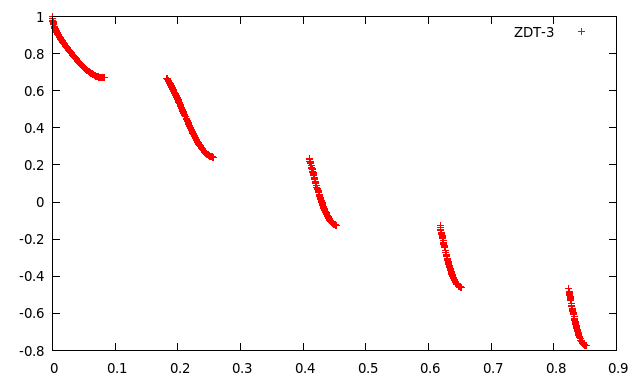
\includegraphics[width=50mm]{zdt3.png}
%   \end{center}
% \end{frame}
% 
% \begin{frame}
%   \frametitle{Implemented Algorithms and benchmark problems 2/2}
%   GA to solve tiled matrix multiplication (TMM)
%   \begin{itemize}
%     \item Accelerated matrix multiplication through better cache utilization (use tiles instead of single row / column)
%     \item Goal: search for optimal tile sizes, such that matrix multiplication times are minimized
%     \item Evaluation of solutions is computed on workers
%     \item Reason for usage: solution evaluation is computational intense $\rightarrow$ low communication overhead
%   \end{itemize}
%   \begin{center}
%     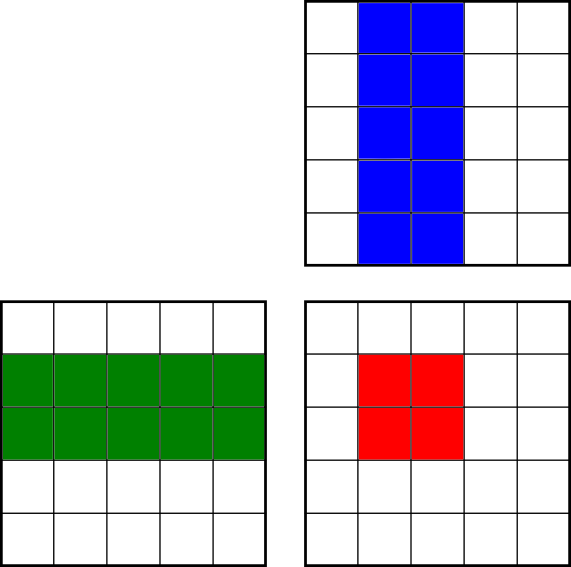
\includegraphics[width=25mm]{tmm.png}
%   \end{center}
% \end{frame}

\begin{frame}
  \frametitle{Correctness of computed results}
  \begin{itemize}
    \item Benchmark results were accurate
    \item ZDT-3: hypervolume as quality indicator showed good results (compared to optimal solution)
    \begin{center}
    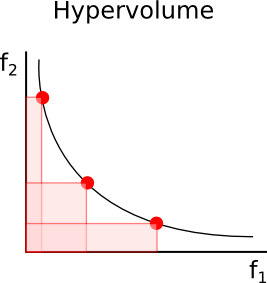
\includegraphics[width=30mm]{hypervolume.png}
  \end{center}
    \item TMM: tiled matrix multiplication provided correct results (compared to simple matrix multiplication)
  \end{itemize}
  
\end{frame}

\begin{frame}
  \frametitle{Performance evaluation}
  \begin{itemize}
    \item Measure algorithm execution time for 1 worker $\rightarrow$ basis for performance evaluation
    \item Increase parallel worker sizes from 1 to 15 to evaluate speedup
    \item Compare parallel execution times to execution time of standalone, sequential algorithm implementation (no Hadoop, no other framework)
  \end{itemize}
\end{frame}
  
\begin{frame}
  \frametitle{Speedups}
  Speedups computed using Amdahl's law: $S = T / (T - t_p)$\\
  \vspace{.5em}
  \scriptsize
  S = Speedup, T = exec. time for 1 worker, $t_p$ = exec. time for p workers
  \begin{columns}
    \begin{column}{.5\textwidth}
      \begin{center}
	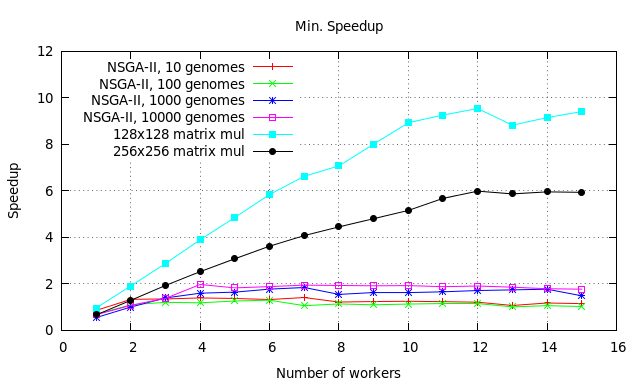
\includegraphics[width=50mm]{speedup_min.png}
      \end{center}
    \end{column}
    \begin{column}{.5\textwidth}
      \begin{center}
	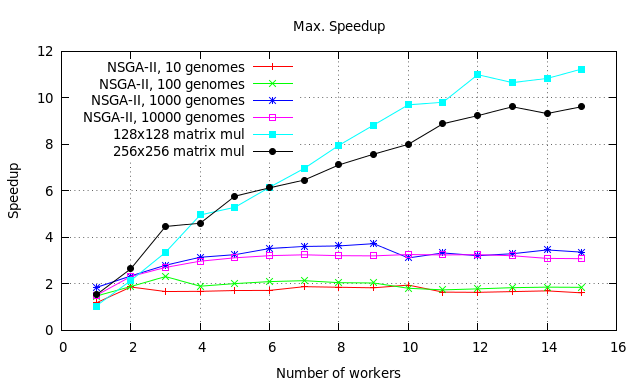
\includegraphics[width=50mm]{speedup_max.png}
      \end{center}
    \end{column}
  \end{columns}
  \normalsize
  \begin{itemize}
    \item Poor ZDT-3 speedups of max \url{~} 4 for 9 workers
    \item Good TMM speedups of max \url{~} 11 for 12 workers
  \end{itemize}
\end{frame}

\begin{frame}
  \frametitle{Comparison to standalone implementations}
  \scriptsize
  \begin{table}
    \centering
%       \caption[Execution times for standalone sequential implementations]{Execution times for $SB$}
    \begin{tabular}{lrrr}\toprule[2pt]
      Test Problem &  Standalone [s] & Parallel [s] & Performance gain \\ \midrule
      ZDT-3, problem size: 10 & 2.852 & 6.461 & 0.441 \\
      ZDT-3, problem size: 100 & 2.956 & 6.128 & 0.482 \\
      ZDT-3, problem size: 1000 & 7.673 & 8.330 & 0.921 \\
      \rowcolor{Gray} ZDT-3, problem size: 10000 & 71.390 & 53.706 & 1.329 \\
      \rowcolor{Gray} TMM, 128$\times$128 & 132.066 & 18.386 & 7.183 \\
      \rowcolor{Gray} TMM, 256$\times$256 & 1500.705 & 178.158 & 8.423 \\ \bottomrule[2pt]
    \end{tabular}
    \label{table:sequential-runtimes}
  \end{table}
  \normalsize
  \begin{itemize}
    \item ZDT-3 performs poor, parallelization has negative impact (except for very big genome sizes)
    \item TMM profits from parallelization
  \end{itemize}
\end{frame}